\begin{titlepage}
\begin{center}

\includegraphics[scale=0.15]{Documents/niser.png}
\line(1,0){300}\\
[2mm]
\begin{large}
\textbf{\huge Adder and Subtractor Circuits}\\ 
\end{large}
\line(1,0){150}\\
[5cm]
\large MAITREY SHARMA\\
\small (1911093)\\
[4.5cm]
Second Year Integrated M.Sc.\\
\textbf{School of Physical Sciences}\\
\textbf{National Institute of Science Education and Research, Bhubaneshwar}\\
\small March 17, 2021
\end{center} 
\end{titlepage}
\newpage
\section{Aim}
\begin{itemize}
    \item To construct half and full adder circuit and verify its working
    \item To construct half and full subtractor circuit and verify its working
    \item To construct a full adder-subtractor circuit
\end{itemize}
\section{Apparatus}
\noindent Digital ICs 7404, 7400, 7408, 7432, 7486 and 7402, resistors, DC voltage source of $\SI{5}{\volt}$, LEDs, breadboard and connecting wires.
\section{Theory}
\noindent
The \textbf{\emph{bit}} is a basic unit of information in computing and digital communications. The name is a portmanteau of \emph{binary digit}. The bit represents a logical state with one of two possible values.
\par
\noindent
An \textbf{\emph{adder}} is a digital circuit that performs addition of numbers. A \textbf{\emph{half}} or \textbf{\emph{single-bit}} adder is where single bits (as the inputs $A$ and $B$) are added together and to get the answer. In half-adder circuits, the carry bit is ignored. But if the carry bit is considered, we can extend our equations to include 2 bits of output. In this case, the half-adder will have 2 outputs, sum $S$ and carry $C$. The simplest half-adder circuit incorporates a XOR gate for $S$ and an AND gate for $C$.
\bigskip
\bigskip
\begin{center}
    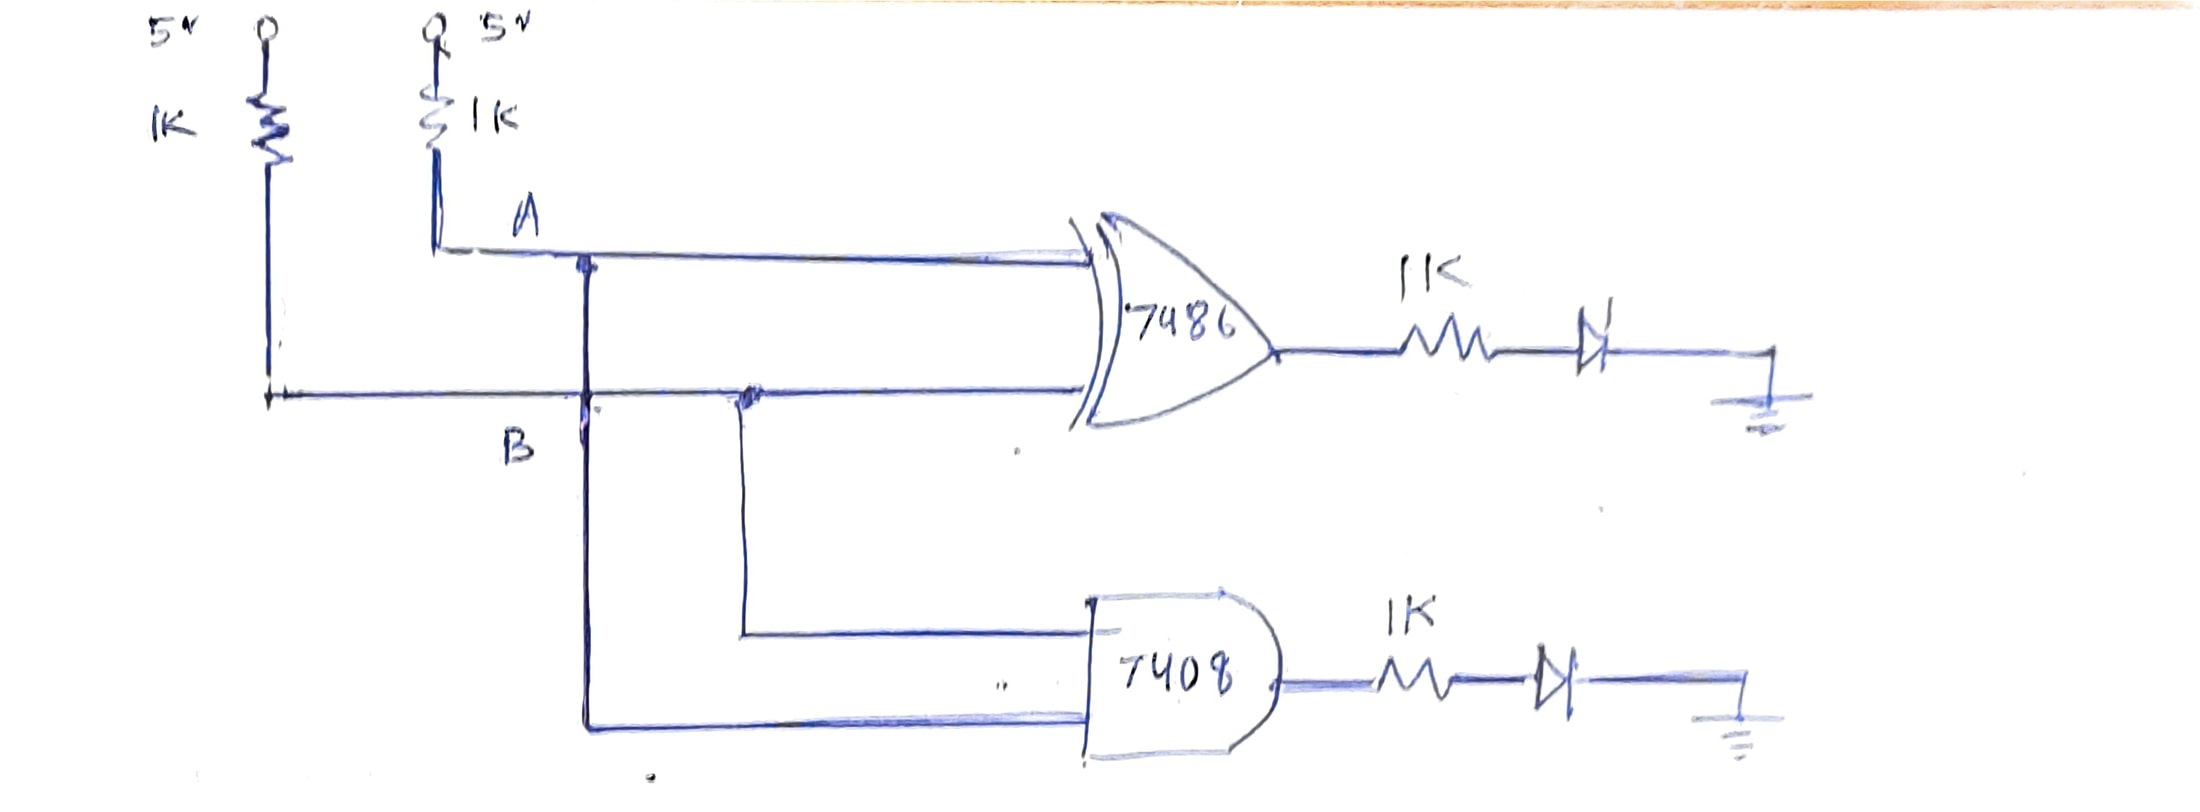
\includegraphics[scale = 0.20]{halfadder_1.jpg}
\end{center}
\begin{center}
    \textbf{The Half-adder Circuit}
\end{center}
\clearpage
\noindent
A \textbf{\emph{full adder}} adds binary numbers and accounts for values carried in as well as out. It accepts inputs $A$ and $B$ plus a carry-in $C_{N-1}$ giving outputs $Q$ and $C_N$. It consists of of two XOR gates, two AND gates and one OR gate.
\begin{center}
    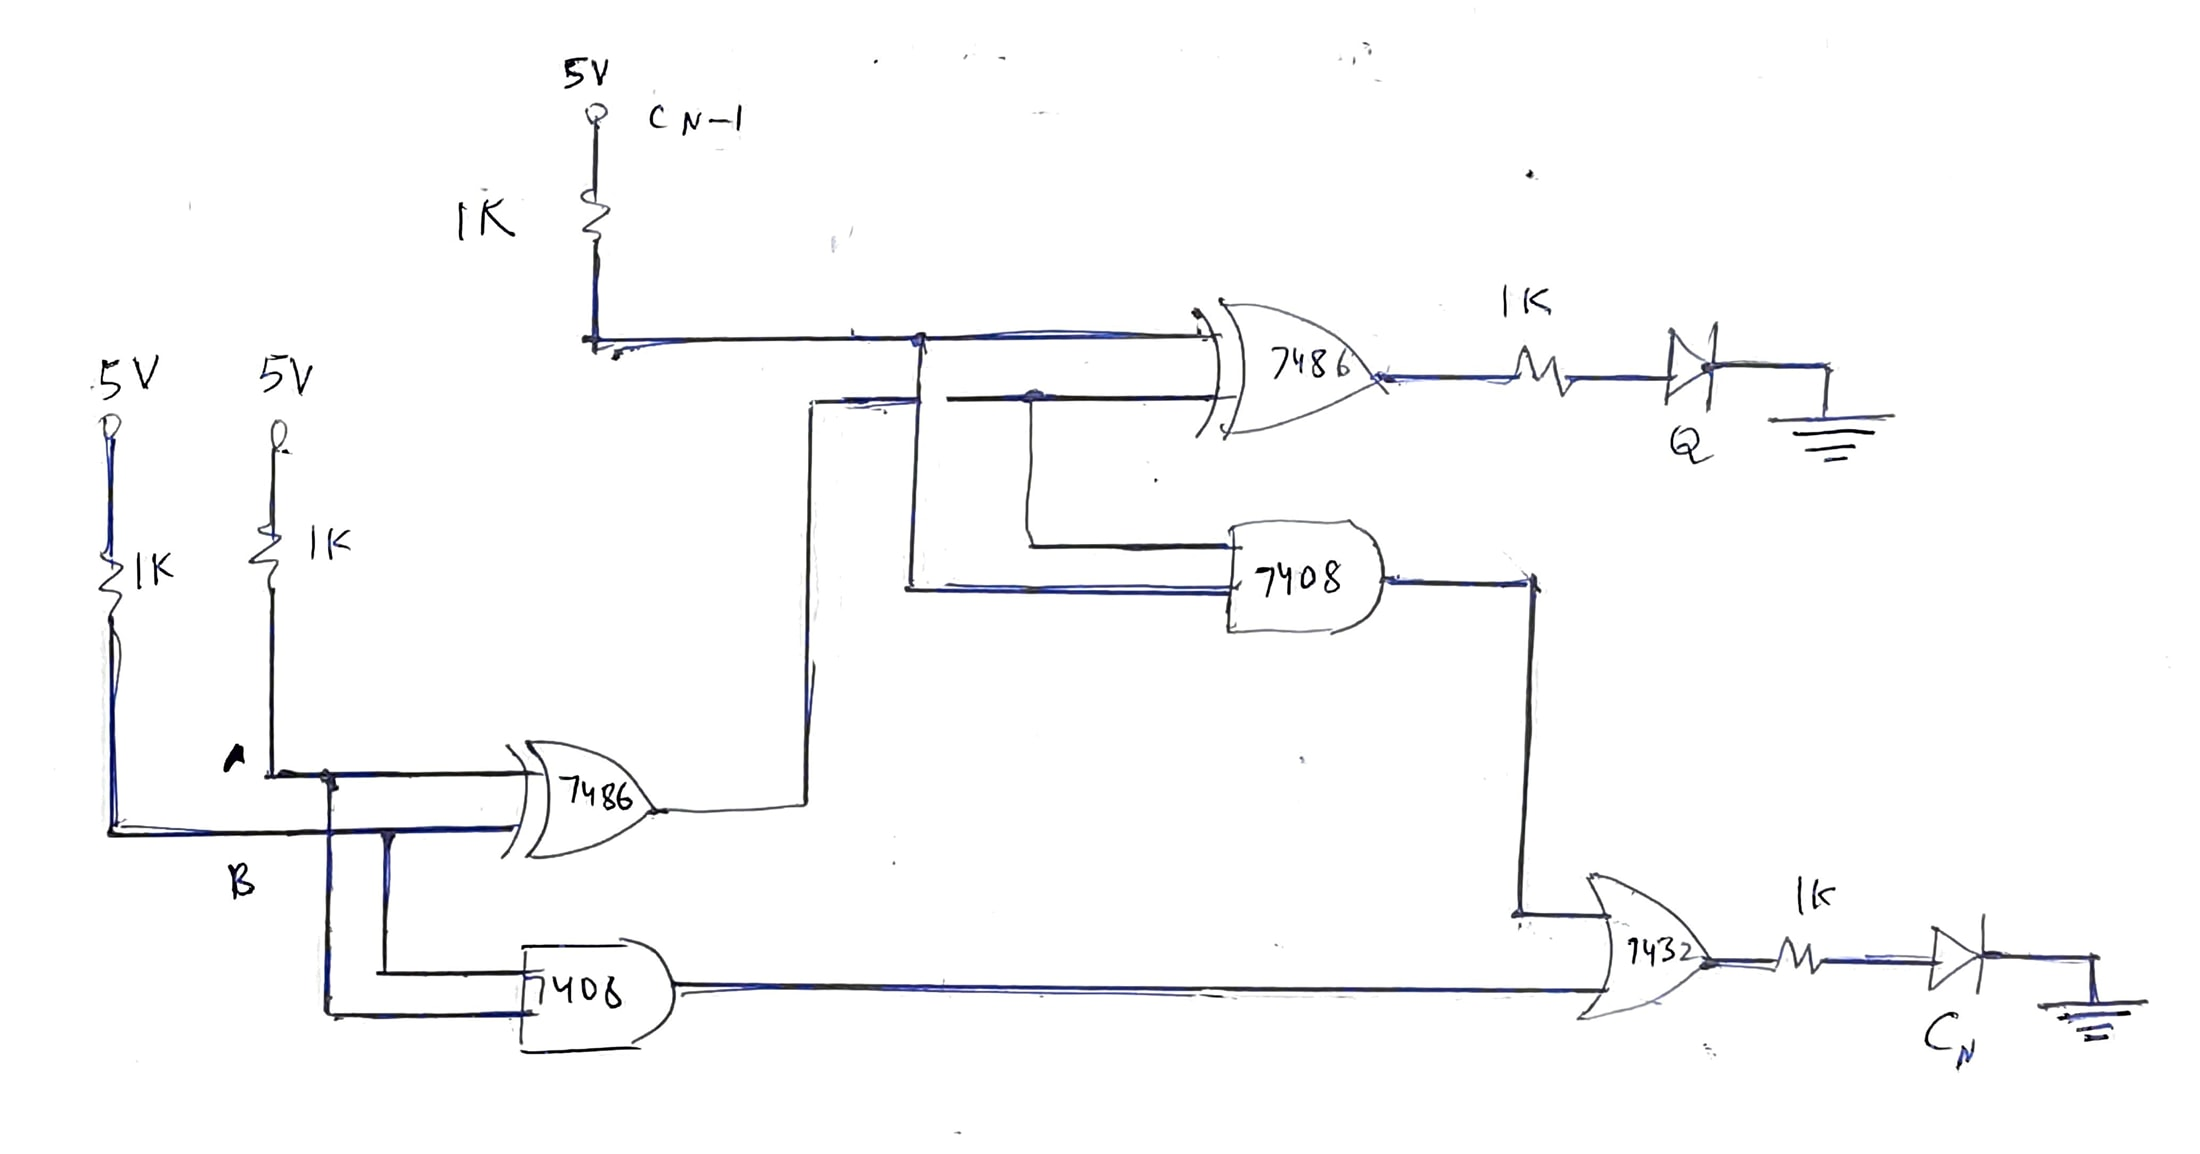
\includegraphics[scale = 0.2]{fulladder_1.jpg}
\end{center}
\begin{center}
    \textbf{The Full-adder Circuit}
\end{center}
The \textbf{\emph{half subtractor}} is a combinational circuit which is used to perform subtraction of two bits. It has two inputs, the minuend $A$ and subtrahend $B$ and two outputs the difference $Q$ and borrow out $B_{N}$.
\begin{center}
    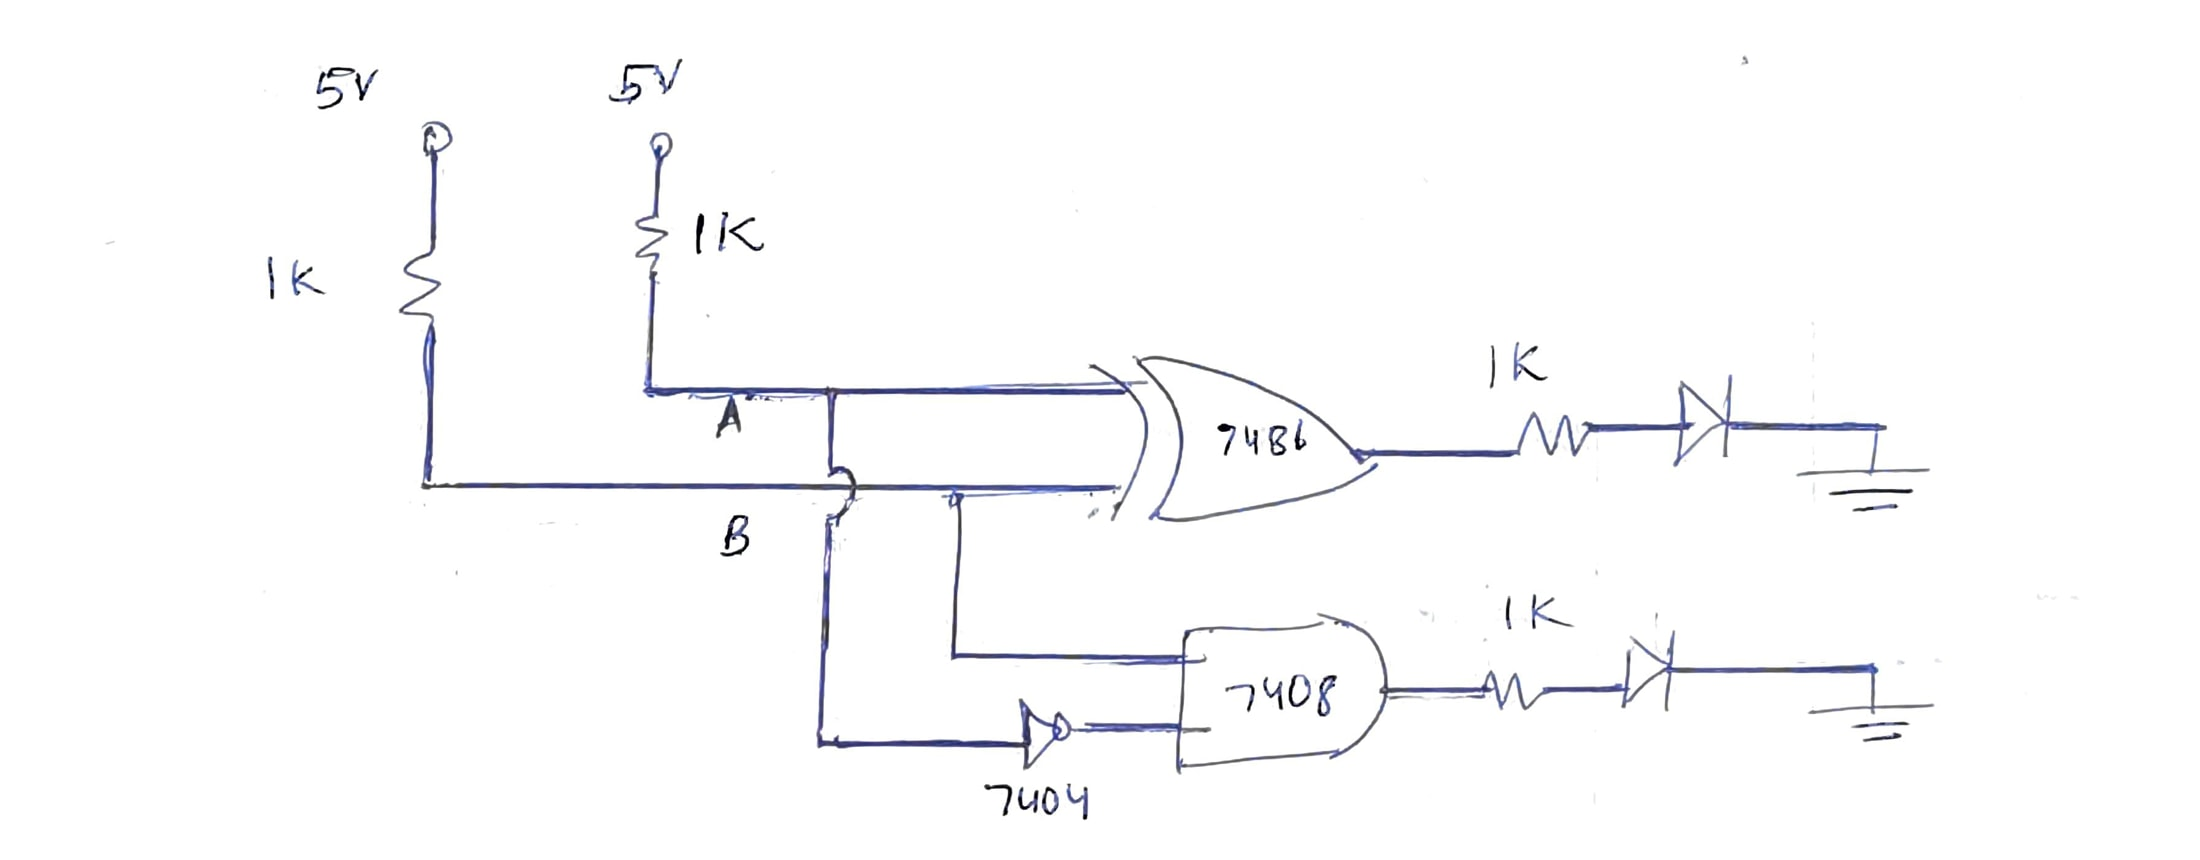
\includegraphics[scale = 0.2]{halfsubtractor_1.jpg}
\end{center}
\begin{center}
    \textbf{The Half-subtractor circuit}
\end{center}
The \textbf{\emph{full subtractor}} is a combinational circuit which is used to perform subtraction of three input bits: the minuend $A$, subtrahend $B$, and borrow in $B_{N-1}$. The full subtractor generates two output bits: the difference $Q$ and borrow out $B_{N}$. $B_{N-1}$ is set when the previous digit is borrowed from $A$.
\begin{center}
    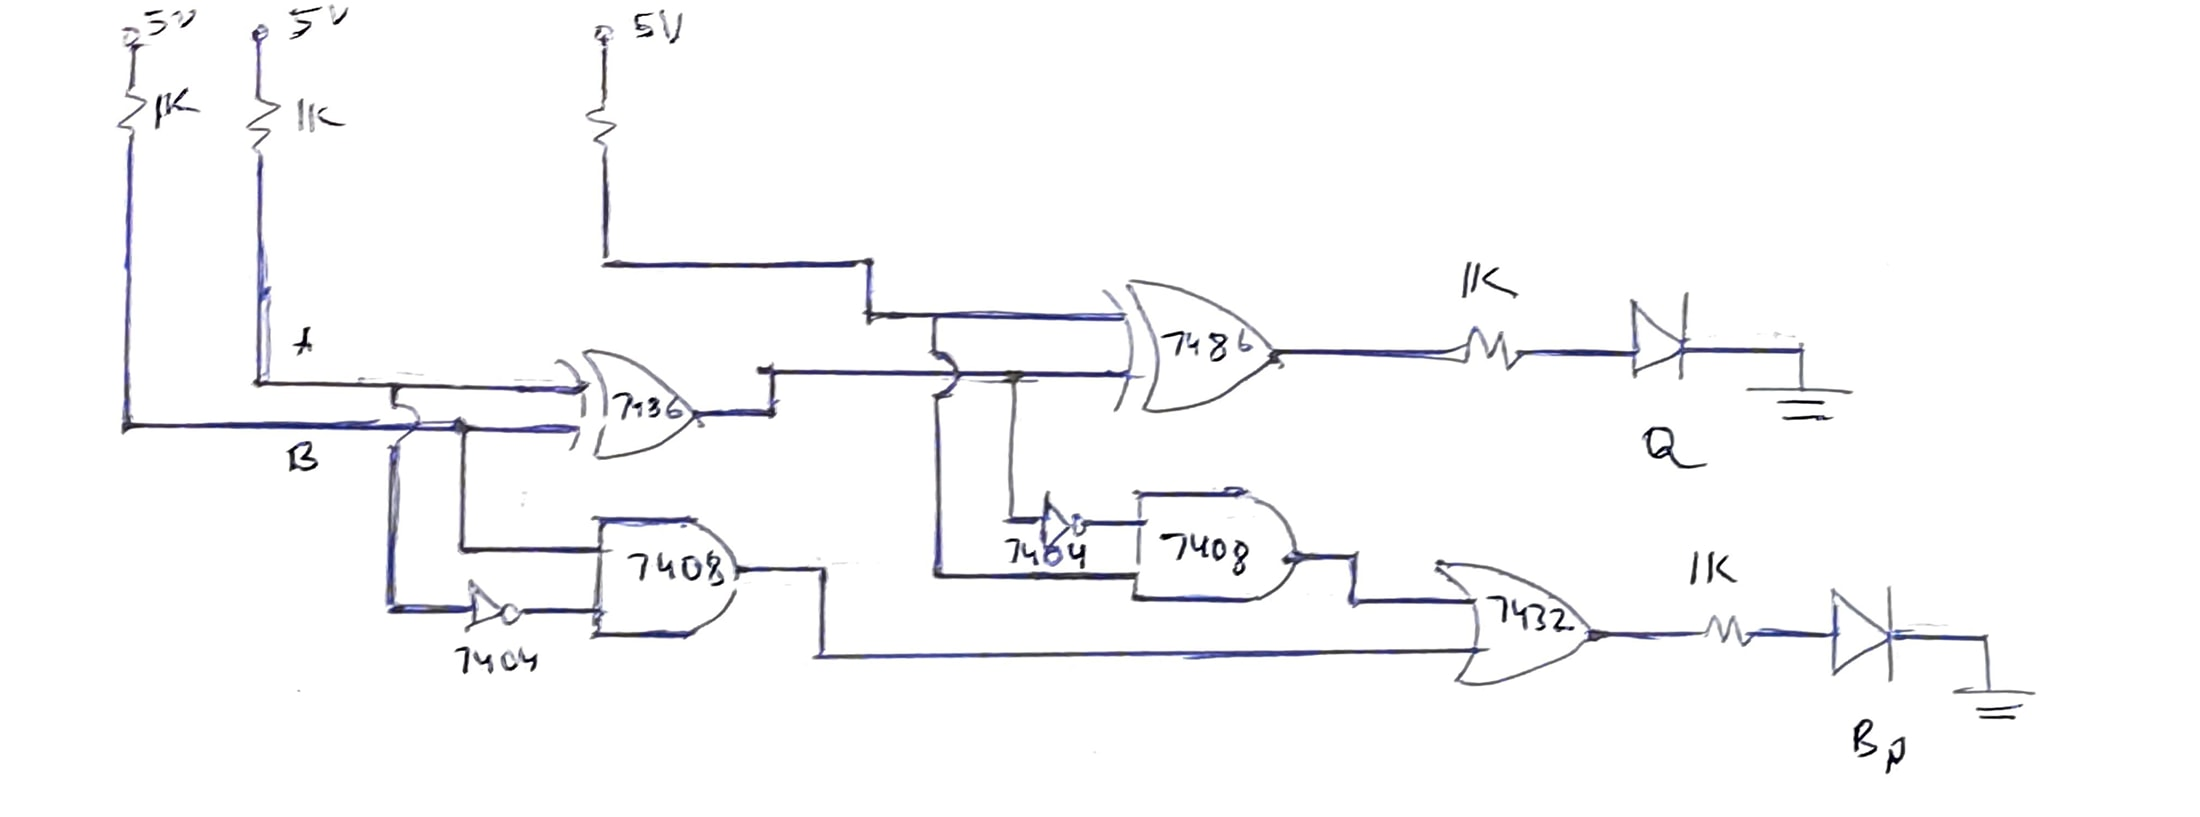
\includegraphics[scale = 0.2]{fullsubtractor_1.jpg}
\end{center}
\begin{center}
    \textbf{The Full-subtractor circuit}
\end{center}
The \textbf{\emph{adder–subtractor}} is a circuit that is capable of adding or subtracting numbers at the same time. It employs two control signals through which it can acts as an adder and subtractor both.
\begin{center}
    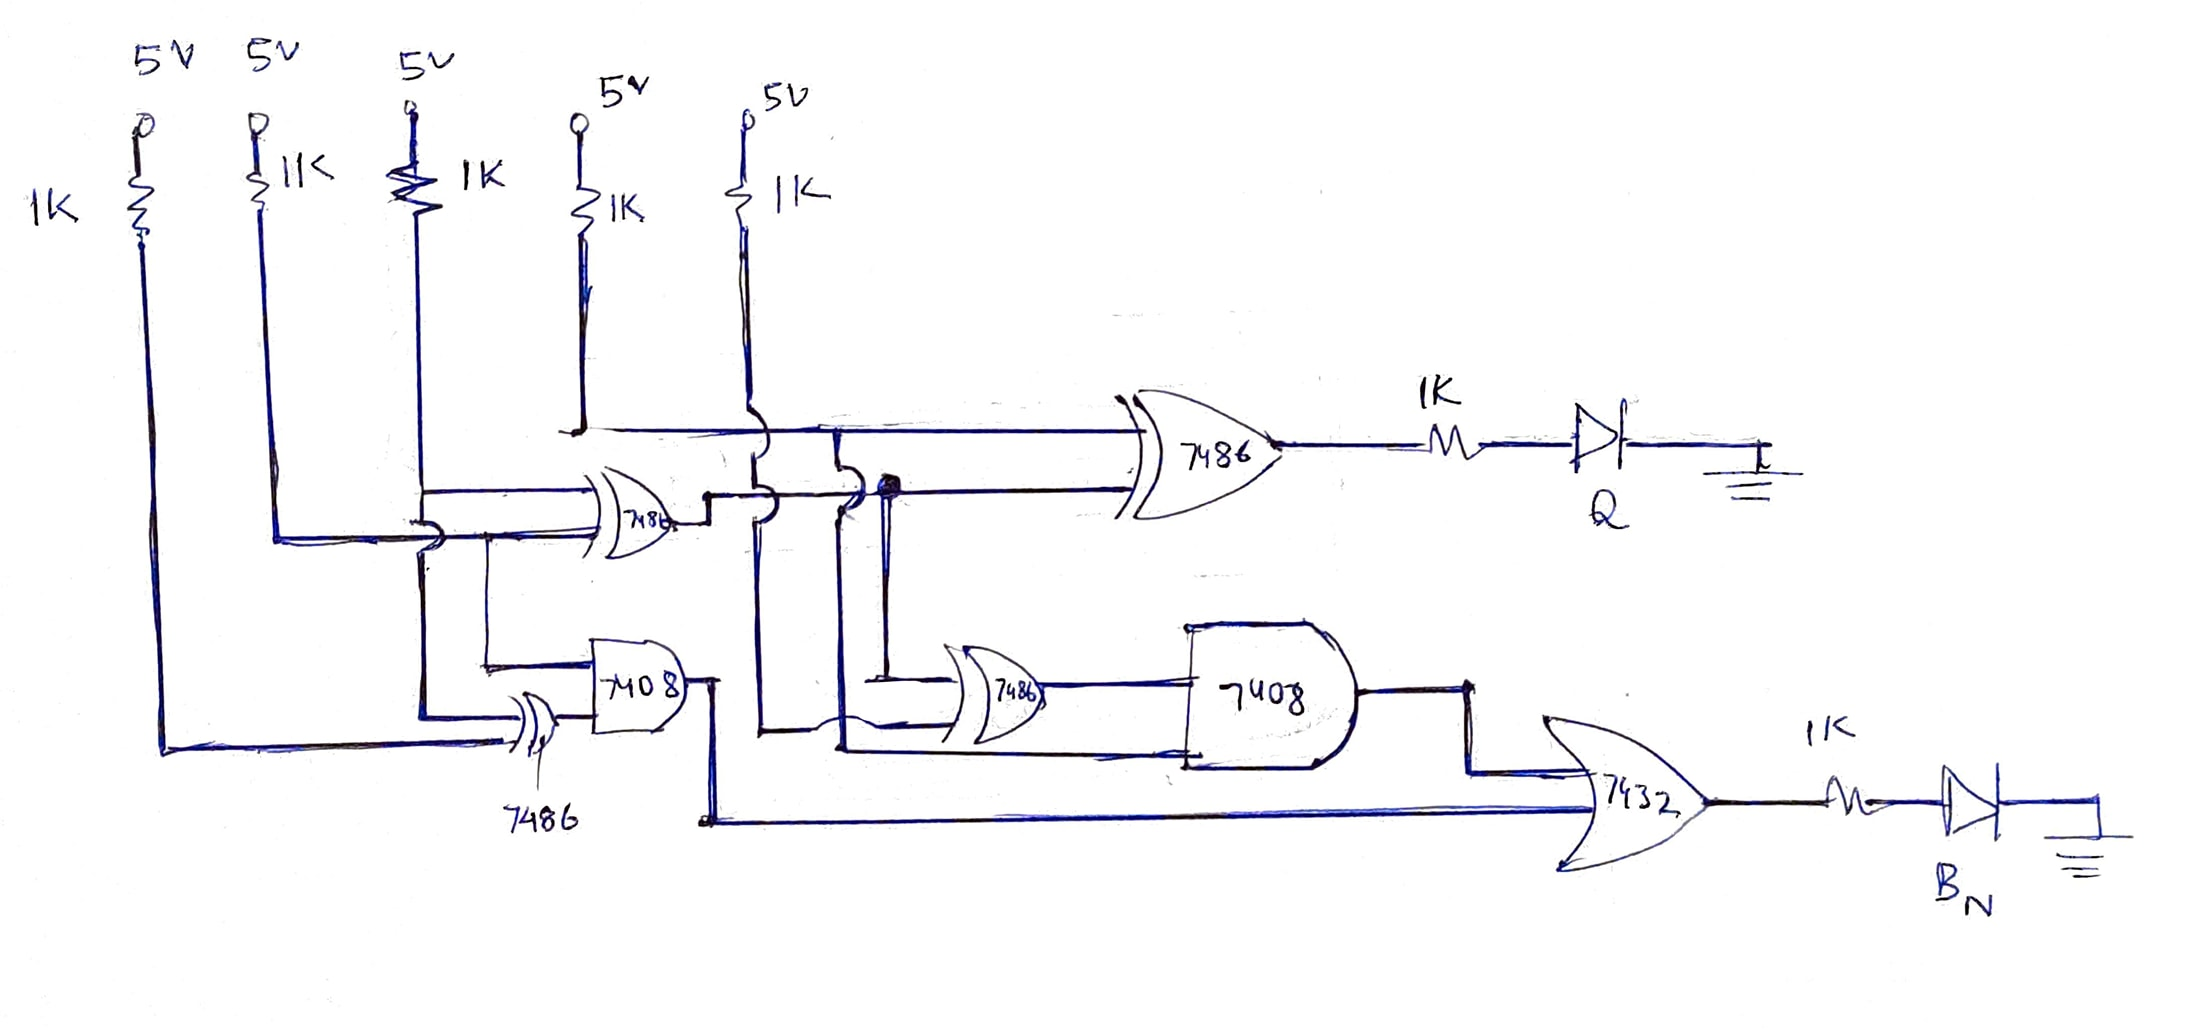
\includegraphics[scale = 0.2]{1615830083100.jpg}
\end{center}
\begin{center}
    \textbf{The Full Adder-Subtractor circuit}
\end{center}
\clearpage
\section{Observations}
\begin{center}
    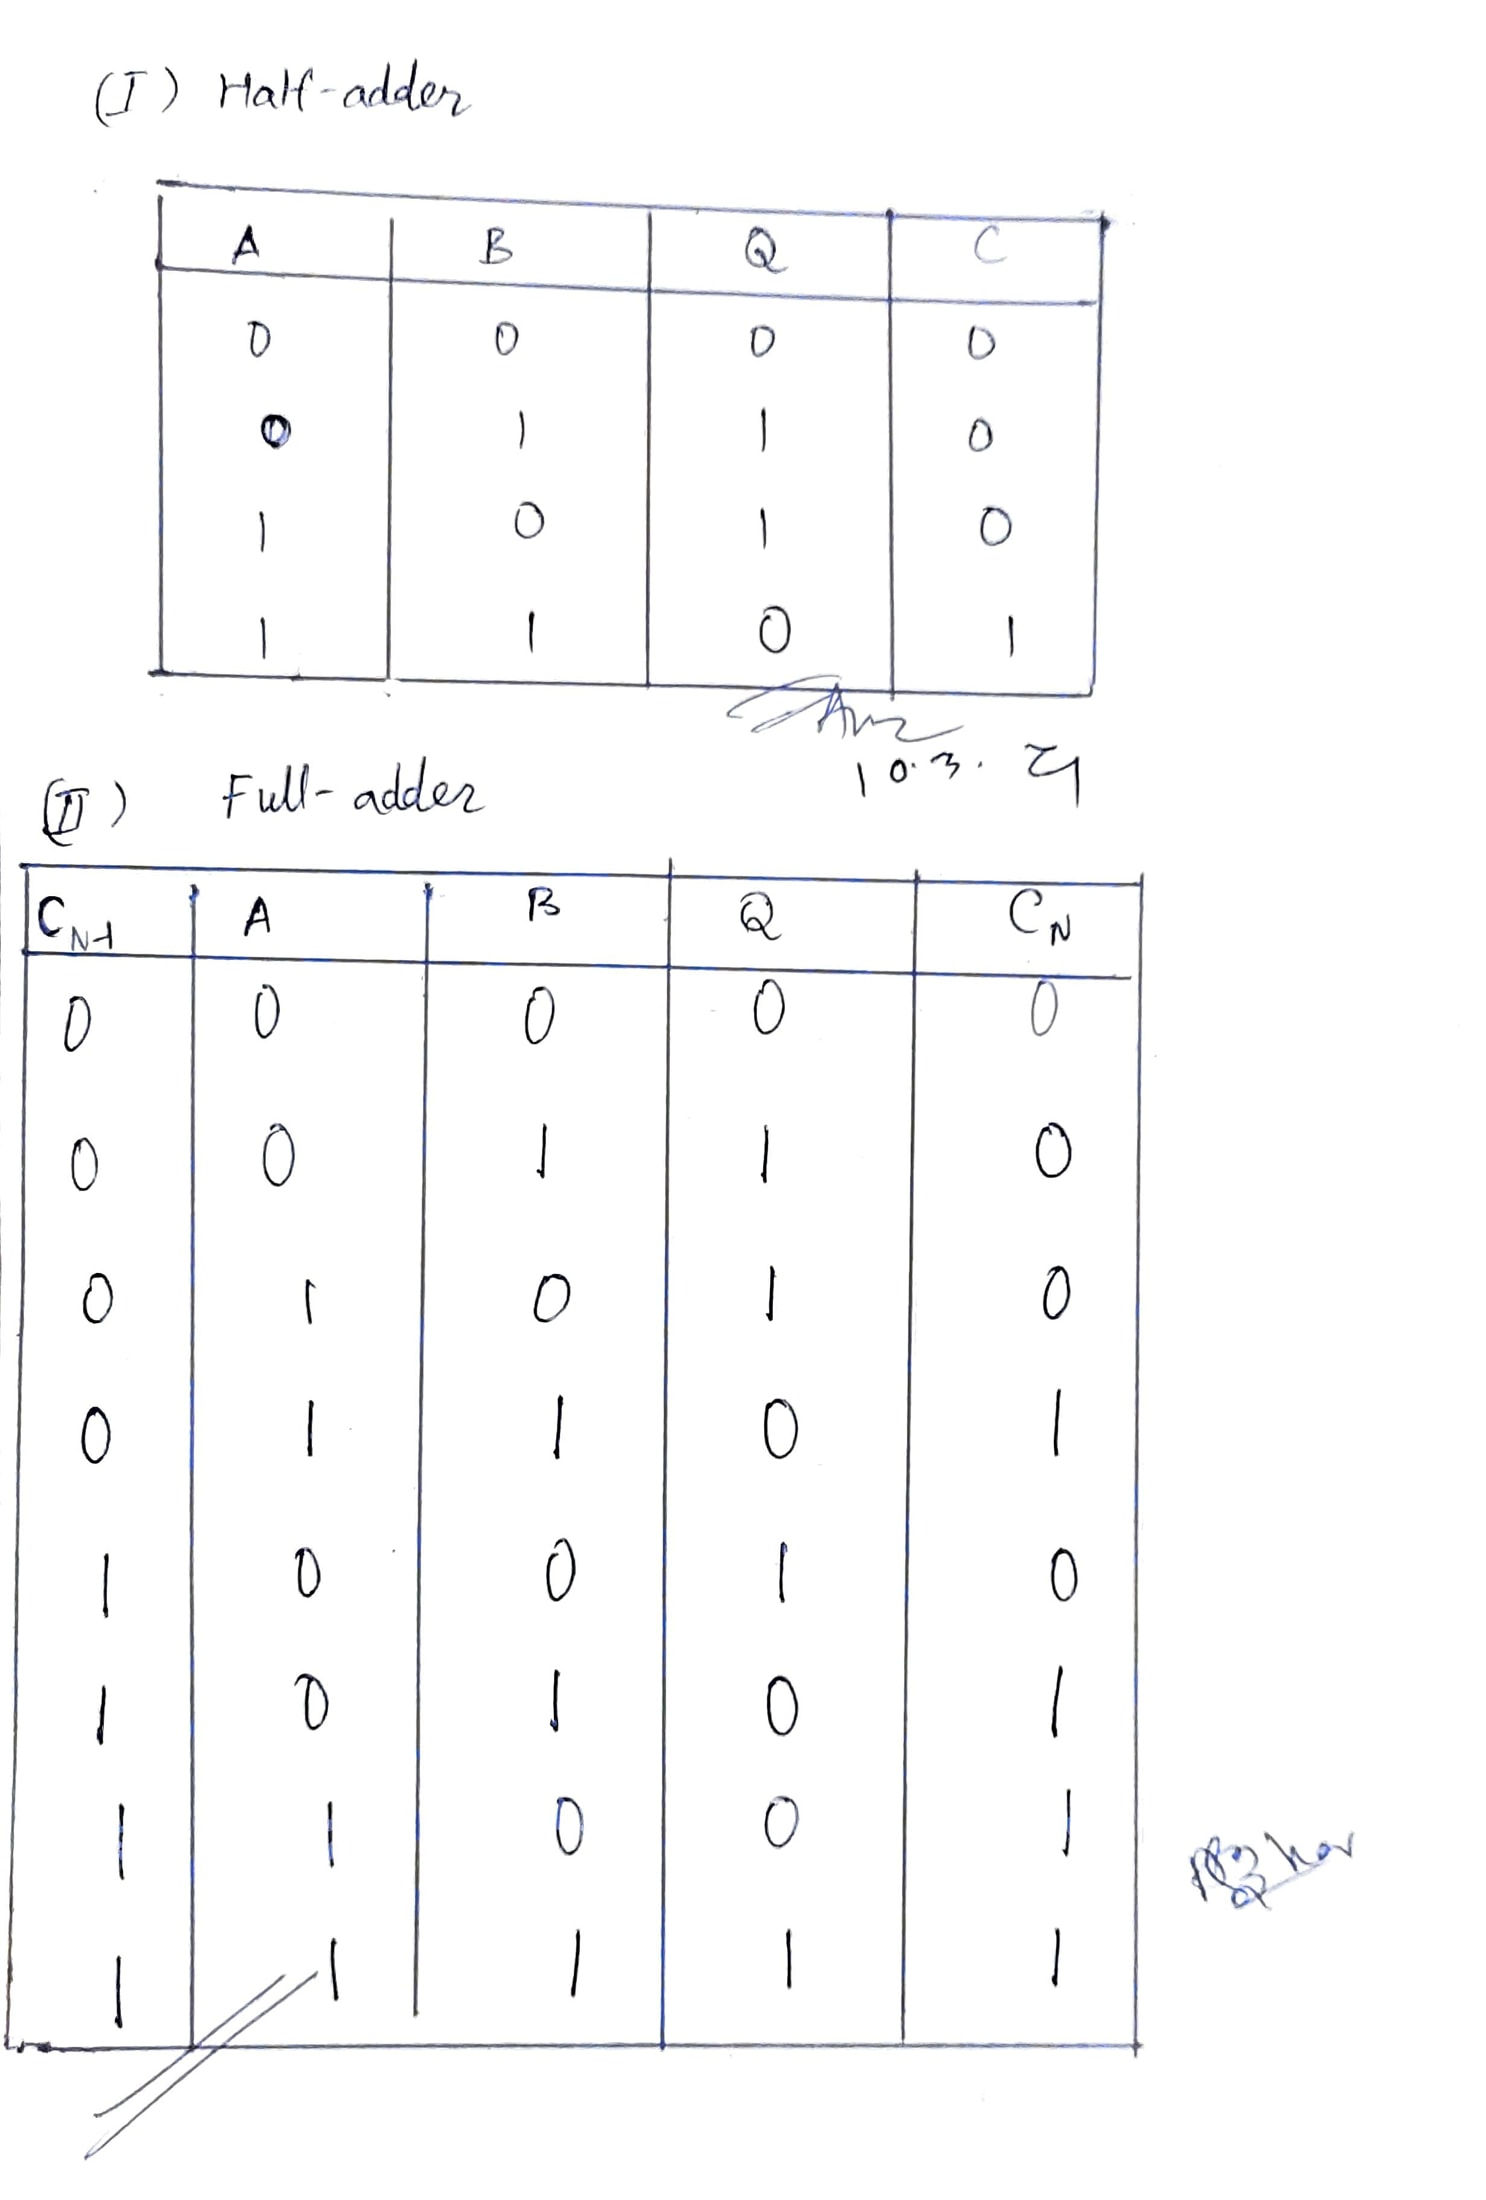
\includegraphics[scale = 0.14]{exp5tab1_1.jpg}
\end{center}
\begin{center}
    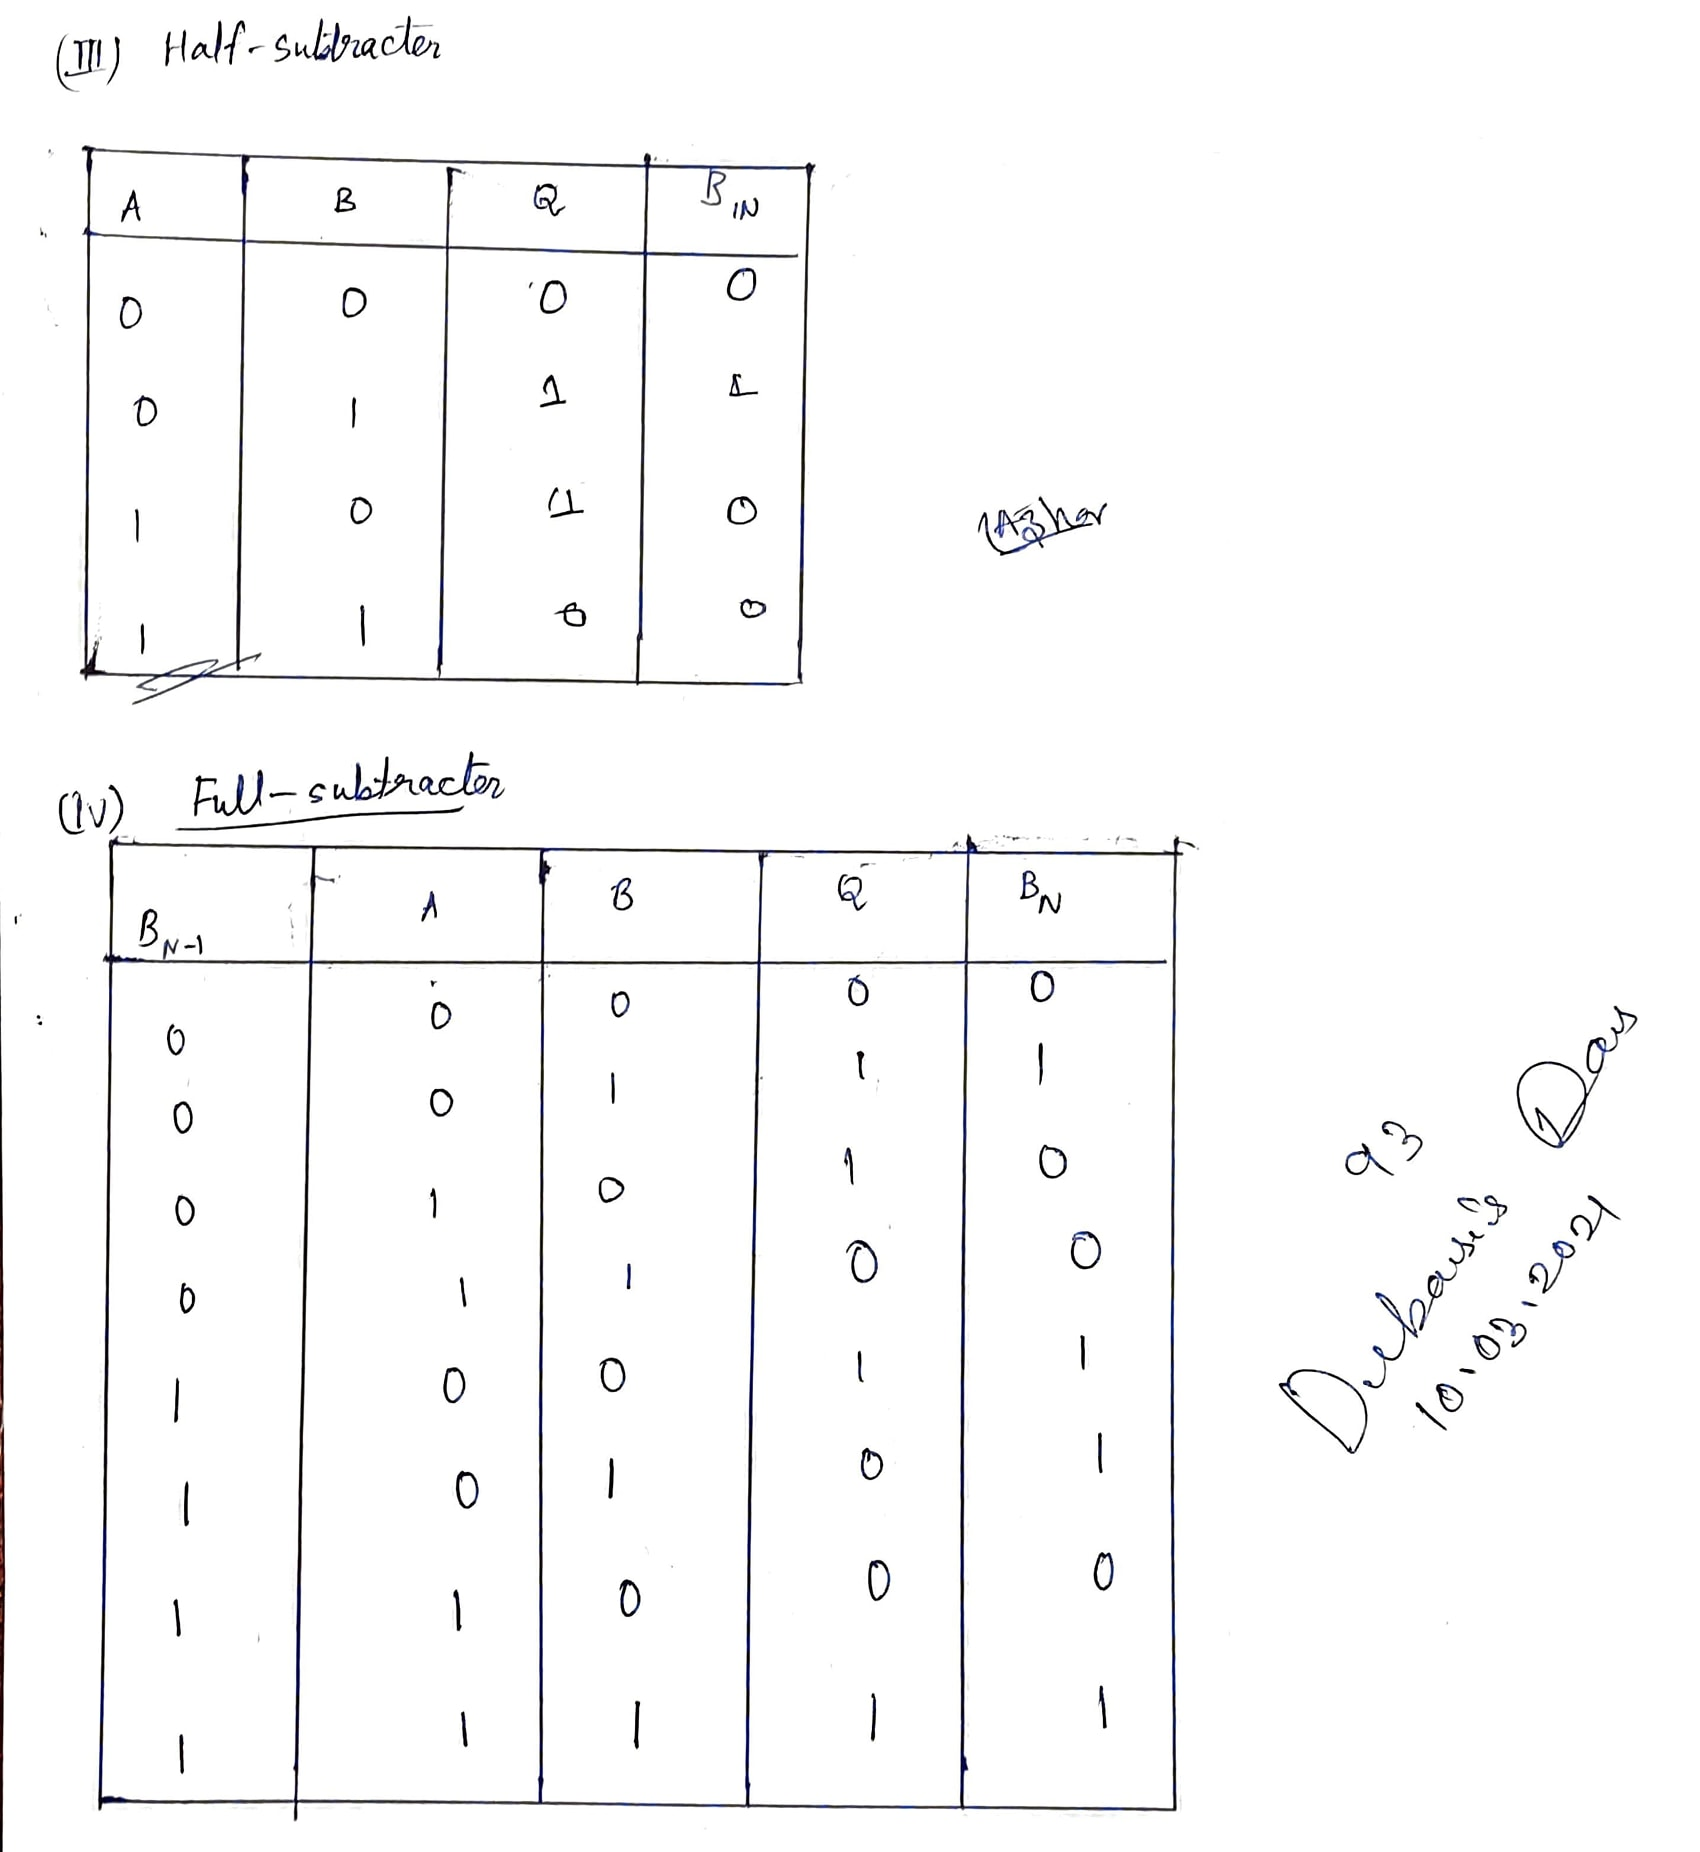
\includegraphics[scale = 0.14]{exp5tab1.5_1.jpg}
\end{center}
\begin{center}
    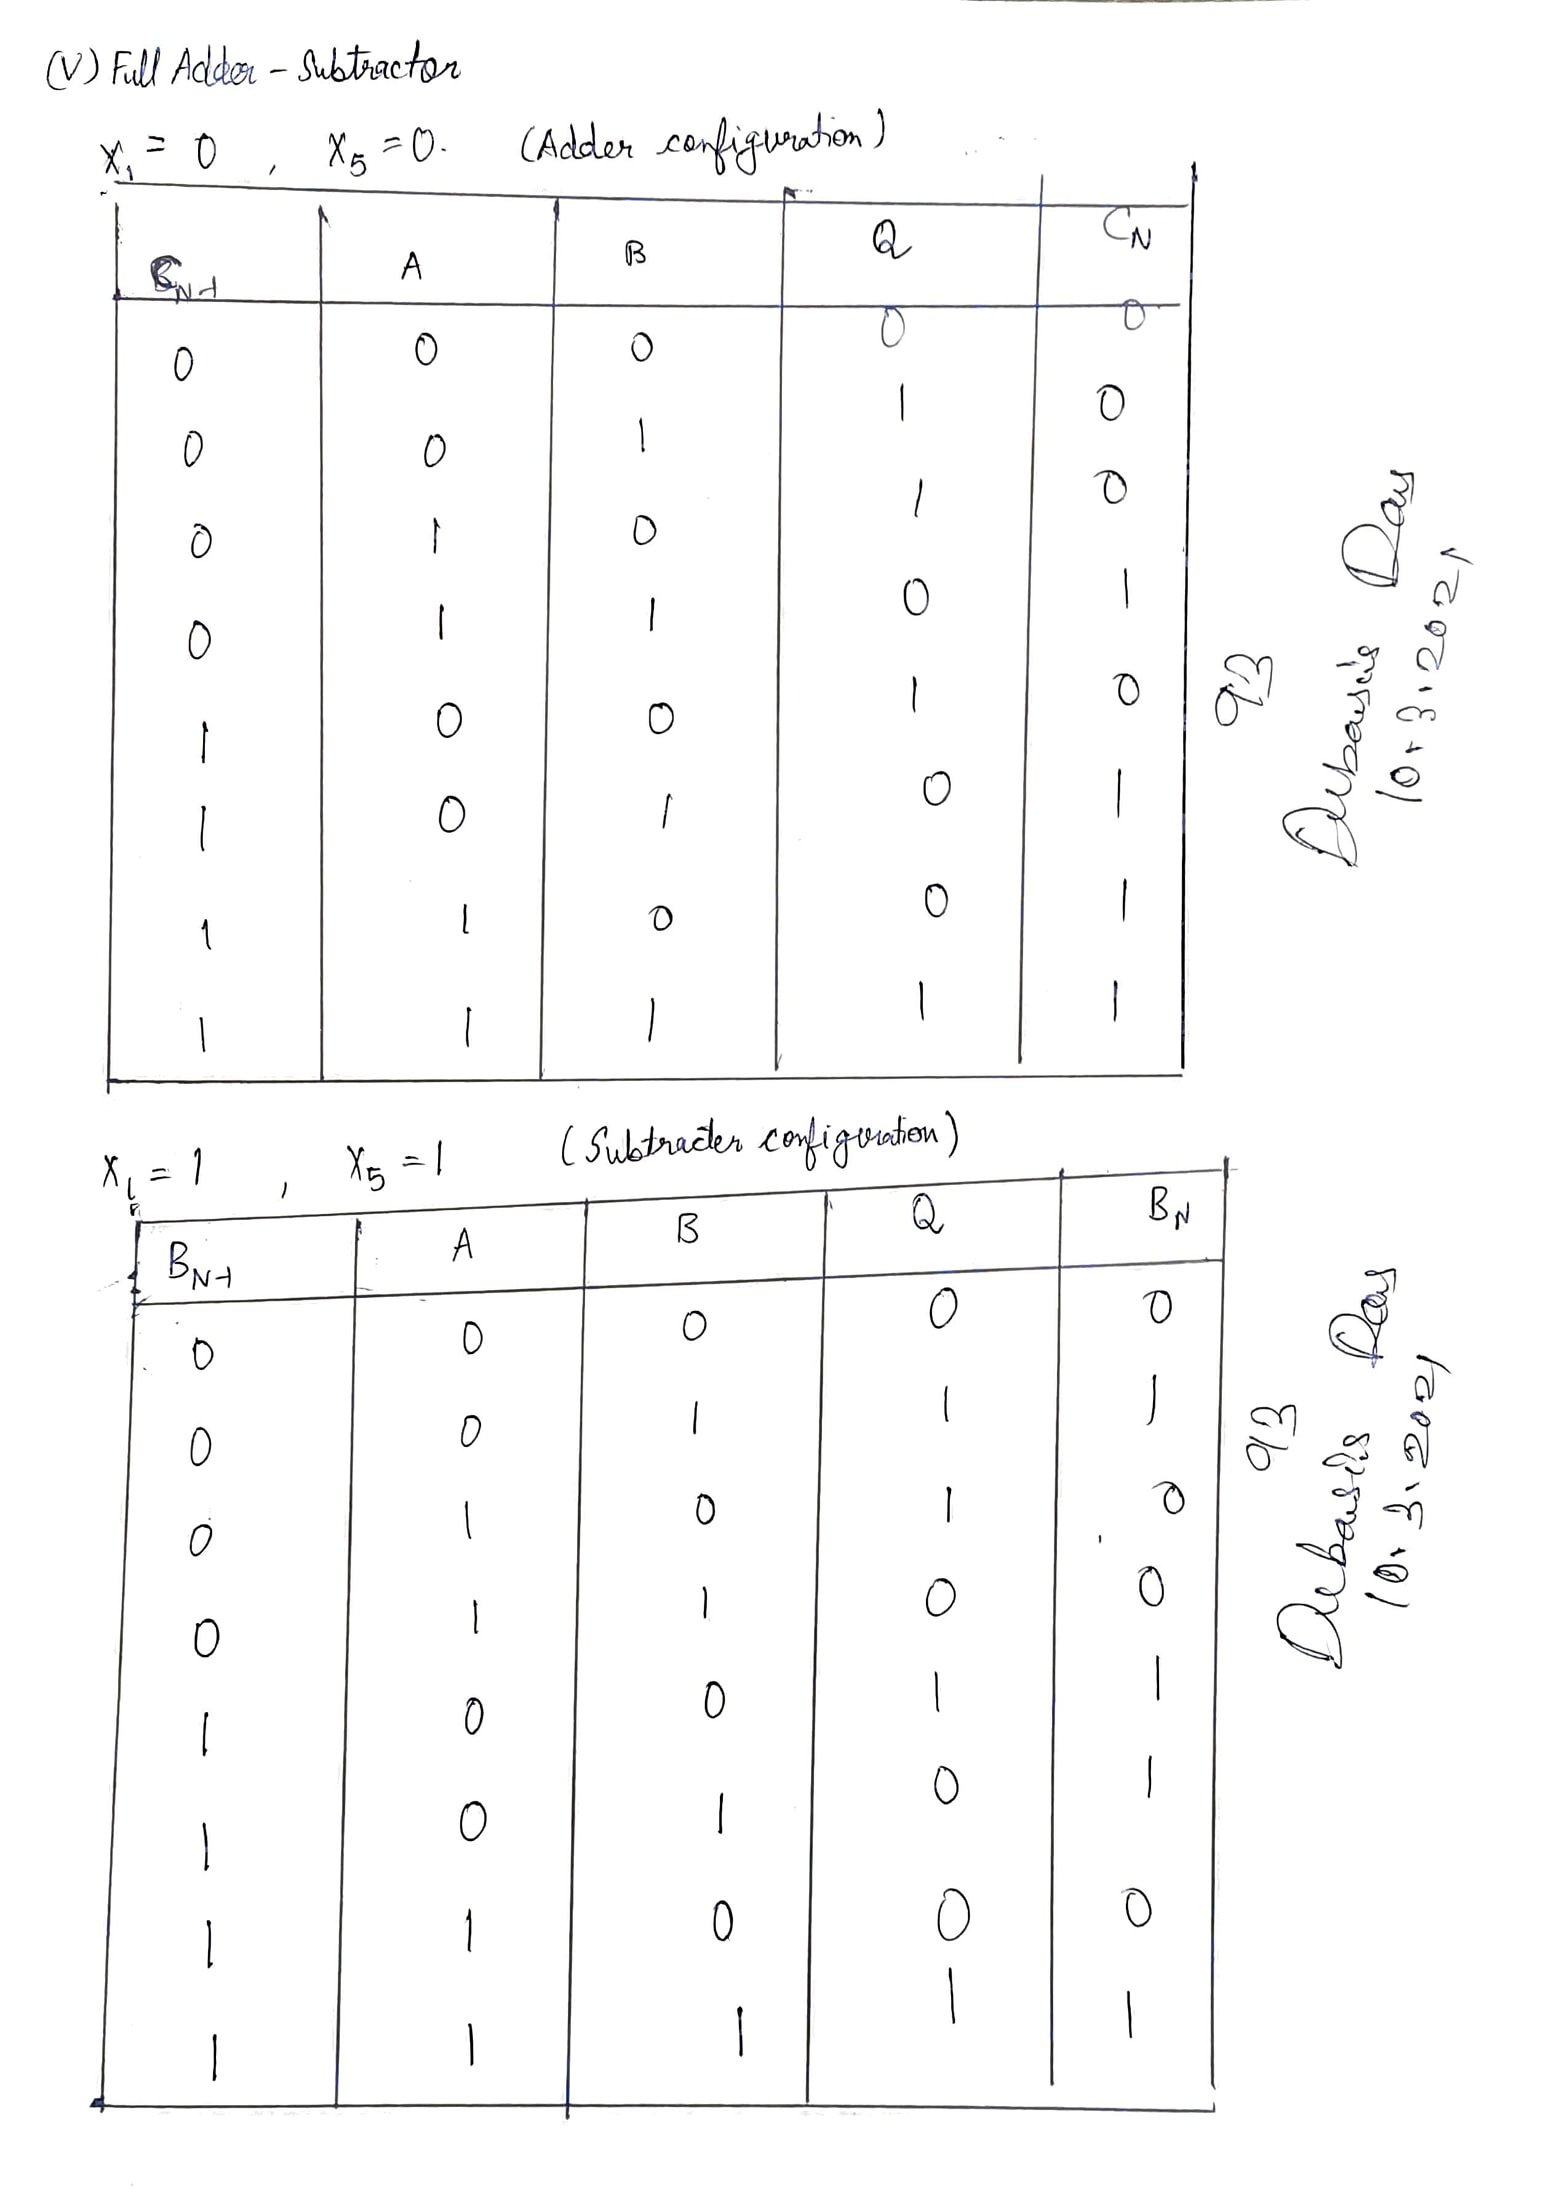
\includegraphics[scale = 0.2]{exp5tab2_1.jpg}
\end{center}
\section{Results}
\begin{enumerate}
    \item The logic gate truth tables are obtained as enumerated under Observations section
\end{enumerate}
\section{Discussions}
\begin{enumerate}
    \item Adders and subtractors are wildly used in in computer’s ALU (Arithmetic logic unit) to compute addition as well as CPU (Central Processing unit) and GPU (Graphics Processing unit) for graphics applications to reduce the circuit complexity. 
    \item Adder and subtractor are basically used for performing arithmetical functions like addition, subtraction, multiplication and division in electronic calculators and digital instruments.
    \item Adders are used in digital calculators for arithmetic addition and devises that uses some kind of increment or arithmetic process
    \item They are also used in microcontrollers for arithmetic additions, PC (program counter) and timers.
    \item It is also used in processors to calculate address, tables and slimier operations.
    \item It is also used in networking and DSP (Digital signal processor) oriented system.
\end{enumerate}
\section{Error Analysis}
\begin{enumerate}
    \item This experiment being a qualitative one, there are no errors per se.
    \item But we can note some precautions such as loose wiring leading to flickering of the LEDs (thus no conclusive "ON" or "OFF" inference.)
\end{enumerate}
\section{Conclusion}
\begin{enumerate}
    \item All results obtained are in accordance to the expectations.
\end{enumerate}